\section{Appendix}

Figures \ref{fig:soap_roc} and \ref{fig:idba_roc} are the ROC plots for all (139 choose 3) enzymes for SOAPdenovo and IDBA assembly of {\em Francisella tularensis}, respectively.  The heat maps give an idea of the probability of getting a particular true positive rate and false positive rate with a specific choice of enzymes.  These plots show the sensitivity and specificity of misassembly detection using optical mapping data alone.  The paired-end sequence data was not used.  As can be seen in the plots, if a set of enzymes were chosen at random then optical mapping would still be informative and produce a meaningful classifier.  

        \begin{figure}[h!]
            \centering
              	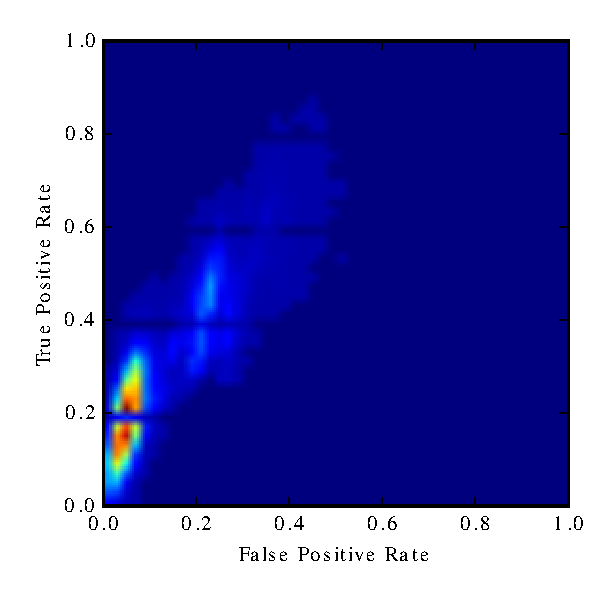
\includegraphics[scale=.9]{./soap.eps}
                	\caption{ROC plot illustrating the density of optical map alignment based missassembly detection classification rates for the SOAPdenovo assembly of {\em Francisella tularensis}. The color intensity at each point indicates the number of three enzyme based classifiers having that classification rate. The plot includes results for optical maps with all three enzyme combinations using a set of 135 enzymes randomly drawn from the REBASE database.  The velvet assembly (which is not shown) has a similar pattern.  Hot spots represent the likely classification rate for enzymes choosen at random.}
                	\label{fig:soap_roc}
        \end{figure}

        \begin{figure}[h!]
            \centering
              	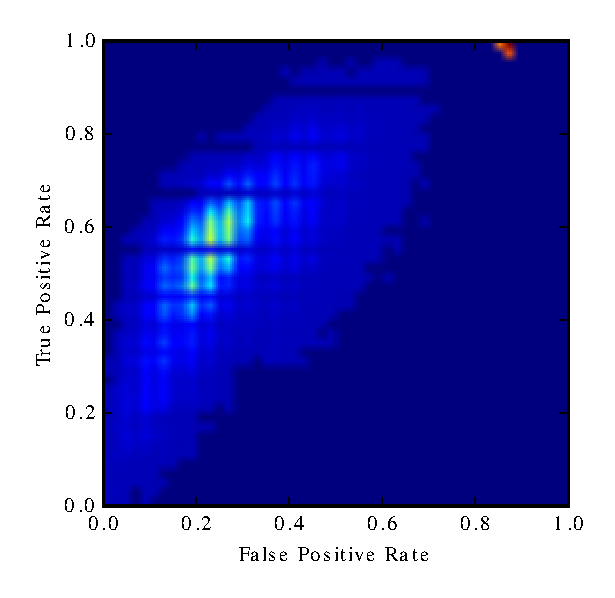
\includegraphics[scale=.9]{./idba.eps}
                	\caption{ROC plot illustrating the density of optical map alignment based missassembly detection classification rates for the IDBA assembly of {\em Francisella tularensis}. The color intensity at each point indicates the number of three enzyme based classifiers having that classification rate. The plot includes results for optical maps with all three enzyme combinations using a set of 135 enzymes randomly drawn from the REBASE database.  Both SPAdes assemblies as well as ABySS (which are not shown) have a similar pattern. Hot spots represent the likely classification rate for enzymes choosen at random.}
                	\label{fig:idba_roc}
        \end{figure}
